% !TEX root = main.tex
% ======================================================================
%  BIBM / IEEE 课程论文模板（支持中英文混排）
%  适用课程：《生物文本挖掘与知识发现》
%  最终稿：基于 PubMed 文献挖掘与水稻性状本体的水稻抗旱基因-性状调控关系发现与可信度审计
%  作者：易子茗（2024317240212，生信2402）
%  编译方式：xelatex -> bibtex -> xelatex -> xelatex
% ======================================================================
\documentclass[conference]{IEEEtran}
\IEEEoverridecommandlockouts

% ---------- 基础宏包 ----------
\usepackage{cite}
\usepackage{amsmath,amssymb,amsfonts}
\usepackage{algorithmic}
\usepackage{graphicx}
\usepackage{textcomp}
\usepackage{xcolor}
\usepackage{url}
\usepackage{booktabs}
\usepackage{tabularx}
\usepackage{multirow}

% ---------- 双栏浮动体排版优化 ----------
\setcounter{dbltopnumber}{2}
\renewcommand{\dbltopfraction}{0.92}
\renewcommand{\dblfloatpagefraction}{0.82}
\setlength{\dbltextfloatsep}{5pt plus 1pt minus 1pt}
\setlength{\textfloatsep}{5pt plus 1pt minus 1pt}
\setlength{\floatsep}{5pt plus 1pt minus 1pt}
\setlength{\dblfloatsep}{5pt plus 1pt minus 1pt}

% ---------- 页码与页脚设置 ----------
\usepackage{fancyhdr}
\pagestyle{fancy}
\fancyhf{}
\fancyfoot[C]{\thepage}
\renewcommand{\headrulewidth}{0pt}
\renewcommand{\footrulewidth}{0pt}

% ---------- 页脚左下角灰色水印（模板要求展示） ----------
\fancyfoot[L]{%
  \scriptsize\color{gray}%
  \begin{tabular}[b]{@{}l@{}}
    课程论文支持使用 Agent 生成内容，\\
    这只是开始。人工内容审查\\
    和驾驭才是终点。%
  \end{tabular}%
}
\setlength{\footskip}{26pt}

% IEEEtran 首页 (\maketitle) 默认使用 plain / IEEEtitlepagestyle，需同步页脚
\fancypagestyle{plain}{%
  \fancyhf{}%
  \fancyfoot[C]{\thepage}%
  \fancyfoot[L]{%
    \scriptsize\color{gray}%
    \begin{tabular}[b]{@{}l@{}}
      课程论文支持使用 Agent 生成内容，\\
      这只是开始。人工内容审查\\
      和驾驭才是终点。%
    \end{tabular}%
  }%
  \renewcommand{\headrulewidth}{0pt}%
  \renewcommand{\footrulewidth}{0pt}%
}
\fancypagestyle{IEEEtitlepagestyle}{%
  \fancyhf{}%
  \fancyfoot[C]{\thepage}%
  \fancyfoot[L]{%
    \scriptsize\color{gray}%
    \begin{tabular}[b]{@{}l@{}}
      课程论文支持使用 Agent 生成内容，\\
      这只是开始。人工内容审查\\
      和驾驭才是终点。%
    \end{tabular}%
  }%
  \renewcommand{\headrulewidth}{0pt}%
  \renewcommand{\footrulewidth}{0pt}%
}

% ---------- 行号设置 ----------
\usepackage[switch]{lineno}
\pagewiselinenumbers

% ---------- 中文支持 ----------
\usepackage[UTF8]{ctex}
\setmainfont{Times New Roman}

\def\BibTeX{{\rm B\kern-.05em{\sc i\kern-.025em b}\kern-.08em
    T\kern-.1667em\lower.7ex\hbox{E}\kern-.125emX}}

\begin{document}

% ======================================================================
%  标题 / 作者 / 单位
% ======================================================================
\title{基于 PubMed 文献挖掘与水稻性状本体的\\抗旱基因--性状调控关系发现与可信度审计}

\author{
\IEEEauthorblockN{易子茗}
\IEEEauthorblockA{
\textit{学号：2024317240212} \\
\textit{华中农业大学信息学院（生信2402）} \\
代码仓库：\url{https://github.com/ZimingADR/BioNLP}}
}

\maketitle

% ======================================================================
%  摘要 / 关键词
% ======================================================================
\begin{abstract}
水稻抗旱基因和表型的实验证据分散在大量论文摘要里，通用医学文本挖掘工具通常缺乏农艺性状词表，也分不清同形基因别名。本文整理了 3,306 篇 PubMed 水稻抗旱摘要（35,345 句、795,401 词元），合并 Oryzabase 的 102,860 条基因别名和水稻性状本体（RTO-1.0）的 3,904 条同义词，用五条农学规则去除冲突简称。全语料一共标出 10,708 处 RAP 水稻基因提及（PubTator 原生映射的 22.6 倍）和 29,966 处性状提及；剔除 1,162 条非水稻或未映射条目后，剩下 7,868 条水稻候选对。随后用 spaCy 依存树计算基因到性状的最短依存路径（SDP），联合论元结构、loss-of-function 极性反转和 \texttt{respectively} 对齐规则，从中抽取 884 条候选因果调控关系（575 条正向、150 条负向、159 条中性，涉及 385 个基因与 693 个唯一基因--性状对），另保留 1,379 条 \texttt{association}。100 条分层人工审计测得 SDP 精确率为 86.0\%（95\% CI: 73.8\%--93.0\%，推算约 760 条真实调控），高于加权共现基线的 34.5\%；极性准确率为 88.2\%（30/34），召回率为 28.0\%。排名前 100 的因果基因在 TO/RTO 背景库中有 53 个条目达到 $q<0.05$（ABA 敏感性富集 10.68 倍），在 RiceMind 中能查到 99 个，但只有 13 个带明确干旱注解，另有 13 个高频候选基因在 RiceMind 里尚无抗逆注释。
\end{abstract}

\begin{IEEEkeywords}
生物自然语言处理, 水稻抗旱性, 最短依存路径, 实体归一化, 水稻性状本体, 知识图谱
\end{IEEEkeywords}

% ======================================================================
%  I. 引言
% ======================================================================
\section{引言 Introduction}

水稻（\textit{Oryza sativa} L.）养活了全球超过一半的人口，干旱则是导致水稻减产最常见的非生物胁迫。过去二十年，围绕脱落酸（ABA）信号、渗透调节和根系构型改良，研究人员已经克隆并验证了大批抗旱基因。不过某个基因究竟提高还是降低了哪项农艺表型，这些结论大多还是分散在几千篇 PubMed 摘要的英文长句里。人工逐篇整理不仅耗时，而且很难把外源转基因研究和本土水稻基因分干净，在别名合并和调控方向判断上也容易出错。

把常用的生物医学文本挖掘工具直接用到水稻领域，常在三个环节上碰壁。首先是检索词覆盖不均：\texttt{rice} 既是水稻，也是常见姓氏和学校简称；同时论文里更常用 \texttt{drought stress} 或 \texttt{drought resistance}，只查 \texttt{drought tolerance} 会漏掉一大块语料。其次是作物表型词表缺失：PubTator 3.0 这类医学预标注接口主要标疾病、基因和化学物，识别不出 \texttt{drought tolerance} 或 \texttt{stomatal resistance} 这类农艺性状 \cite{wei2024pubtator3}。第三则是基因命名混乱和同形词冲突，同一基因在不同论文里常写成 \texttt{SNAC1}、\texttt{OsNAC9} 或 \texttt{ONAC2}，而常见生理缩写 \texttt{ABA}、产量单位 \texttt{ha-1} 以及对照品种 \texttt{Apo} 又刚好和突变体别名撞名。除此之外，同句共现并不算因果调控，表达相关性、否定修饰和 \texttt{respectively} 并列句都会产生不少假阳性。

为了解决上面这些具体问题，本文把文献检索、词典清洗、句法抽取和知识库核查串成了一套四阶段流程。前期先用物种学名加 MeSH 条件收齐 3,306 篇 PubTator 全文，拿多尺度型例比（TTR）和 TF-IDF 二元短语反查检索式是否漏检；中期合并 Oryzabase 基因词典和 RTO-1.0 性状词典，用五条规则拦掉激素、世代与单位简称，再只留以 \texttt{Os} 开头的水稻位点共现。到了关系抽取一步，共现对并没有直接当作调控，而是用 spaCy 的最短依存路径（SDP）去卡主动、被动、名词化和链式论元结构，加入功能缺失（loss-of-function）极性反转与 \texttt{respectively} 配对检查，然后抽 100 条做分层人工审计。最后取排名前 100 的因果基因做 TO/RTO 超几何富集和 RiceMind 比对，检验功能聚集度并找出库里漏标抗逆注释的候选基因。

% ======================================================================
%  II. 相关工作 Related Work
% ======================================================================
\section{相关工作 Related Work}

生物医学文献挖掘一般按照文献获取、实体归一化、关系抽取和知识验证这几步推进 \cite{zhao2021bionlp}。Cancer-Alterome 通过检索 PubMed、整合词典和编写句法规则，从论文里抽取癌症突变调控事件 \cite{canceralterome2024}；PubTator 3.0 提供了面向基因、疾病和化学物质的预标注接口 \cite{wei2024pubtator3}；NLTK 和经典信息检索教材则给出了英文分句、Heaps 定律检查和 TF-IDF 主题计算的常用做法 \cite{nltk2009,manning2008ir,slides2026}。不过，这套医学管线直接用到水稻上时，基因符号体系和农艺性状词表都得重新补齐。

好在水稻领域已经有了比较扎实的参考数据库。Oryzabase 和 RAP-DB 整理了 CGSNL 标准基因名、历史别名与物理位点编号（RAP ID）\cite{kurata2006oryzabase,sakai2013rapdb}；水稻性状本体（RTO-1.0）把植物性状本体（TO）和常见农艺表型组织成受控词表 \cite{rto2026}；RiceMind 则收集了水稻文献挖掘和多组学注释结果 \cite{ricemind2024}。在句法关系抽取方面，RelEx 等工作说明，不依赖大规模人工标注语料时，依靠依存树上的最短依存路径（SDP）依然能较准确地抓住调控动词和主宾角色 \cite{fundel2007}；至于抽出基因集在功能上是否集中，通常用超几何检验配合 Benjamini--Hochberg（BH）校正来做富集评价 \cite{ashburner2000,huang2009,benjamini1995bh}。

和以往只停留在共现统计或者单靠医学 NER 的做法不同，本文把农学五重消歧、loss-of-function 极性反转以及 \texttt{respectively} 错配排除串到同一套流程里，并用 100 条分层审计和 RiceMind 缺口比对把误差范围标清楚，避免把未清洗的共现对误当成确定调控关系。

% ======================================================================
%  III. 数据与方法 Data and Methods
% ======================================================================
\section{数据与方法 Data and Methods}

\subsection{语料检索、限流获取与偏移校验 Data}
为了让检索尽量全、同时压低 \texttt{rice} 当作作者姓氏或机构名带来的杂音，我们在 PubMed 上把检索字段限制在标题、摘要和 MeSH 主题词：
\begin{center}
\vspace{-2pt}
\footnotesize\ttfamily ("Oryza sativa"[Title/Abstract] OR "Oryza sativa"[MeSH Terms]\\
OR "rice"[Title/Abstract]) AND "drought"[Title/Abstract]
\vspace{-2pt}
\end{center}
该检索式命中 3,311 篇文献。脚本调 PubTator 的 \texttt{export/pubtator} 接口逐篇抓取标注，每次请求停顿 \texttt{time.sleep(5.8)} 防止限流，中途支持断点续传，最后解析出 3,306 篇文献。还有 5 篇 2026 年刚上线、PubTator 暂未索引的文献（PMID \texttt{42880016}、\texttt{42881188}、\texttt{42884139}、\texttt{42884770}、\texttt{42884918}），用 PubMed \texttt{efetch} 补好题录和摘要存在 \texttt{unindexed\_pmids.tsv} 里，不计入主统计。照着讲义格式 \cite{slides2026} 把标题与摘要拼为 \texttt{text = title + " " + abstract} 之后，逐条核查 PubTator 原生 47,157 处实体的字符偏移 \texttt{text[b:e] == mention}，47,156 处完全吻合（99.998\%）。只有 PMID \texttt{40588031} 的化学物 \texttt{all-trans-$\beta$-carotene} 因希腊字母编码差异没通过，不影响基因和性状抽取。

\subsection{双词典构建与五重农学消歧 Preprocessing}
为了补上医学 NER 缺失的水稻基因和作物表型维度，本文分别从 RTO-1.0 与 Oryzabase 建立两套词典。性状端遍历 RTO-1.0 里的全部 \texttt{[Term]} 节点，删掉带 \texttt{is\_obsolete} 标记的废弃词和过泛的顶层抽象词，整理出 2,022 个标准性状节点和 3,904 条可匹配同义词。比如 \texttt{drought resistance} 会统一归到 \texttt{drought tolerance}（\texttt{TO:0000276}），\texttt{stomatal closure} 归到 \texttt{stomatal resistance}（\texttt{TO:0000522}）。

基因端读取 Oryzabase 的 22,023 条记录，优先绑定标准 RAP ID（15,862 条），缺 RAP ID 的回退到 Oryzabase ID（6,386 条）。直接拆原表同义词会带进大量噪音，所以加了五条规则做过滤：1) 对 CGSNL 首列为 \texttt{\_} 的 6,000 多条基因，删掉占位符后改用第一个有效同义词作展示名；2) 用正则 \texttt{\textbackslash(t\textbackslash)\textbackslash*?} 剥掉 \texttt{Hd6(t)*} 里的暂定标记，免得拆出单字母 \texttt{t} 别名；3) 把 \texttt{ABA}、\texttt{AsA}、\texttt{JA}、\texttt{ROS}、\texttt{MDA}、\texttt{CAT}、\texttt{SOD} 等生理缩写放进黑名单，防止和冷门突变体撞名；4) 拦掉 \texttt{M1}--\texttt{M5}、\texttt{BC1}、\texttt{B2}、\texttt{B3} 等育种世代代号，以及孤立出现的 \texttt{MYB}、\texttt{WRKY}、\texttt{NAC} 泛称；5) 明确屏蔽产量单位 \texttt{t ha-1} 中的 \texttt{ha-1}（语料里和 \texttt{AHA8} 别名撞了 50 次）以及常见旱稻品种 \texttt{Apo}（和 \texttt{APO} 撞了 47 次）。清理后留下 102,860 条基因别名映射。

\subsection{词汇计量与句子级共现基线 Lexical and Co-occurrence}
把语料转成小写并去掉纯标点后，设词元序列为 $W=(w_1,\dots,w_N)$，独立词型集合为 $V(W)$，原始型例比记为 $\text{TTR} = |V(W)|/N$。按照 Heaps 定律 $|V(N)| \approx K N^{\beta}$ \cite{heaps1978}，窗口越大 TTR 越低。为了拆开看“文本变长”和“单篇摘要用词重复”两个因素，我们在窗口 $k \in \{10^3, 5\times 10^3, 10^4, 5\times 10^4, 10^5, 5\times 10^5\}$ 上比较顺序截断 $\text{TTR}_{\text{head}}(k)$ 和 10 次跨文献随机抽样（\texttt{seed=42}）均值 $\text{TTR}_{\text{shuf}}(k)$：
\begin{equation}
\begin{aligned}
\text{TTR}_{\text{head}}(k) &= \frac{|V(w_{1:k})|}{k}, \\
\text{TTR}_{\text{shuf}}(k) &= \frac{1}{M}\sum_{m=1}^{M}\frac{|V(\mathcal{S}_m(W,k))|}{k}.
\end{aligned}
\label{eq:ttr}
\end{equation}
同时对满足文档频次 $DF(t) \ge \max(2, 0.005|D|)$ 的单字词和二元短语 $t$，按平滑逆文档频率和篇内归一化词频之和计算全语料 TF-IDF 权重 \cite{manning2008ir}：
\begin{equation}
\begin{aligned}
IDF(t) &= \ln\!\left(\frac{1+|D|}{1+DF(t)}\right)+1, \\
\text{Score}(t) &= \sum_{d\in D}\frac{f_{t,d}}{|d|}\cdot IDF(t).
\end{aligned}
\label{eq:tfidf}
\end{equation}

在句子级抽取阶段，程序调用 \texttt{sentence\_spans(text)} 切出 35,345 个句子并保留字符跨度 $[b_{s_i}, e_{s_i})$ \cite{slides2026,nltk2009}。每个句子按 $k=4\to 1$ 最长 $n$-gram 优先扫描，只要命中基因或性状词典，且对应区间没有被 PubTator 非基因实体（如化合物、疾病）掩码占用，就记下绝对坐标。同一句话里只要同时出现至少一个基因和至少一个性状，就输出候选共现对。全语料一共产生 9,030 条候选，但其中 1,162 条指向大豆 \texttt{GmGolS} 等外源或未映射基因；为了让后续网络严格留在水稻单物种范围内，程序按 \texttt{RAP ID} 以 \texttt{Os} 开头做过滤，把最终输入阶段三的水稻候选收口为 7,868 条。

\subsection{基于最短依存路径（SDP）的因果与极性抽取 Methods}
单句共现会把“表达变化”“相关分析”和“并列错配”混进调控关系里。本文用 \texttt{spaCy en\_core\_web\_sm} 对全部水稻候选句做依存句法分析 \cite{honnibal2020spacy}。先把基因和性状的字符跨度对齐到名词短语中心词，再在无向依存图上算出两者的最短路径 $P=(u_0,\dots,u_L)$，沿路径和支配动词选出谓词 $v$。候选对要进入因果判定，必须符合四类基因到性状论元结构之一：一是主动结构，基因在 $v$ 的 \texttt{nsubj} 或 \texttt{nsubjpass} 子树内，性状落在 \texttt{dobj}、\texttt{attr} 或 \texttt{to/of/for} 介词宾语上；二是被动结构，性状作 \texttt{nsubjpass} 而基因落在 \texttt{by}-agent 短语里；三是名词化构建，如 \texttt{overexpression/knockout of GENE} 作主语去支配性状宾语；四是链式从句，$v_1$ 主语含基因，$v_2$ 处在 $v_1$ 的补足语或关系从句中去支配性状。

判断调控方向时，程序结合正/负/中性谓词词表、程度副词和依存否定修饰；如果基因主语子树带有功能缺失构建词（如 \texttt{knockout}、\texttt{silencing}、\texttt{mutation}、\texttt{inactivation}、\texttt{repression}），规则会自动把谓词极性取反，这样“敲除导致耐旱性下降”就能正确还原成该基因正向调控耐旱。遇到含 \texttt{respectively} 的句子时，程序按基因与性状在句中的出现序号配对，序号对不上的标记为 \texttt{excluded\_respectively}。所有候选最终分成三类因果（\texttt{positive\_regulation}、\texttt{negative\_regulation}、\texttt{regulation}）、补充关联层 \texttt{association}、\texttt{no\_effect}、\texttt{excluded\_direction}、\texttt{excluded\_respectively} 和 \texttt{unsupported}，并按路径长度、论元模式和极性明确度标上 \texttt{high}/\texttt{medium}/\texttt{low} 置信度。

\subsection{分层人工审计、TO/RTO 富集与 RiceMind 验证 Evaluation}
为了评估规则的实际准确率并估算漏检比例，我们固定 \texttt{seed=42} 抽取 100 条做分层审计。A 层从 884 条预测因果中随机取 50 条，用来算精确率与 Wilson 95\% 置信区间 \cite{wilson1927}；B 层从 6,984 条非因果里按类别配额取 50 条（\texttt{association} 20 条、\texttt{excluded\_direction} 15 条、\texttt{excluded\_respectively} 5 条、\texttt{no\_effect} 5 条、\texttt{unsupported} 5 条），再按 A/B 两层总体规模加权推算召回率、$F_1$ 以及共现基线精确率。标注只看句子里有没有写清“某个基因（或其过表达、敲除、突变体）改变了对应性状”：写清了就按正、负或方向未明记成 $+1$、$-1$ 或 \texttt{reg}；只提表达变化、相关系数、别的性状，或者实体认错，全标为 $0$。这 100 条先由作者和辅助 Agent 做过一轮预标，后面又逐条人工核对修改，属于单团队核查样本，尚无多位植物学专家双盲独立标注。

功能富集部分把 SDP 因果证据数排前 100 的水稻基因作为查询集（$k=100$，全部落在背景库内），在 RiceMind 与文献拼成的背景基因集（$N=2{,}218$ 个基因、272 个 TO/RTO 条目）上算单侧超几何上尾概率，再用 BH 方法做多重校正 \cite{huang2009,benjamini1995bh}：
\begin{equation}
p_j = \Pr(X \ge x_j \mid N, m_j, k) = \sum_{i=x_j}^{\min(m_j, k)} \frac{\binom{m_j}{i}\binom{N-m_j}{k-i}}{\binom{N}{k}},
\label{eq:hyper}
\end{equation}
以 $q_j < 0.05$ 为显著富集。随后查询 RiceMind 的 \texttt{gene-profile} 接口看这 100 个基因的 \texttt{trait\_class} 与 \texttt{annotation} 内容，凡是已有至少 3 个唯一 SDP 因果对、在 RiceMind 中却没有 \texttt{stress/tolerance} 注释的，均标为待审编的注释缺口候选；所有唯一因果对还被汇总成一张无向加权二分网络。

% ======================================================================
%  IV. 结果 Results
% ======================================================================
\section{结果 Results}

\subsection{语料规模、多尺度 TTR 与 TF-IDF 检索反证}
解析后的 3,306 篇文献共包含 35,345 个句子（每篇平均 10.69 句）、795,401 个词元和 34,247 个独立词型，全语料原始 TTR 为 4.31\%。从图~\ref{fig:lexical}(a) 可以看到，随着窗口从 1,000 词元扩到全量，词型从 542 个增长到 34,247 个，原始 TTR 从 54.20\% 降到 4.31\%，符合 Heaps 定律的幂律衰减曲线。再看图~\ref{fig:lexical}(b) 里顺序截断和全局随机抽样的差值：在 $1\text{k}$--$50\text{k}$ 窗口下，shuf 均值比 head 高 1.62--2.42 个百分点（$N=10{,}000$ 时是 28.90\% 对 26.48\%），到 $500\text{k}$ 时就缩小到 0.23 个百分点。这说明样本还不大时，跨篇随机抽样能更好避开单篇摘要反复出现同一批术语造成的偏差。

\begin{figure*}[t]
  \centering
  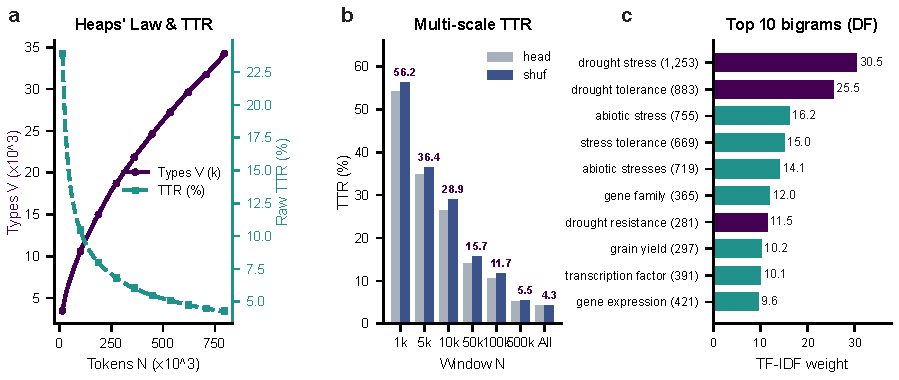
\includegraphics[width=0.95\textwidth]{figure/fig1_lexical_tfidf.pdf}
  \caption{水稻抗旱语料（3,306 篇、795,401 词元）的词汇统计与检索词覆盖分析。(a) 词型数 $V(N)$ 与原始 TTR 随语料长度的 Heaps 定律变化；(b) 七个窗口尺度下顺序截断（head）与 10 次随机抽样（shuf）TTR 对比；(c) Top 10 TF-IDF 二元短语及其文档覆盖篇数（DF）。数据来源：\texttt{part1\_lexical\_and\_tfidf\_summary.json}。}
  \label{fig:lexical}
\end{figure*}

TF-IDF 排名反映了整个语料的核心研究主题。单字词里除 \texttt{drought}（$DF=3{,}079$，得分 64.88）和 \texttt{stress}（$DF=2{,}535$，61.18）外，\texttt{genes}（1,829）、\texttt{tolerance}（1,731）、\texttt{expression}（1,684）、\texttt{yield}（896）、\texttt{root}（605）和 \texttt{aba}（589）排在最前，串起了逆境信号、基因表达到器官与产量的研究链条。图~\ref{fig:lexical}(c) 的二元短语排名给出了一项直接的检索依据：\texttt{drought stress}（TF-IDF 30.5）覆盖了 1,253 篇文献，比 \texttt{drought tolerance}（883 篇）多出 370 篇（多覆盖 41.9\%），而 \texttt{drought resistance} 又占了 281 篇。如果当初只用 \texttt{rice AND drought tolerance} 去查库，大约会漏掉三分之二的相关文献。

\subsection{双词典归一化消融与异构别名汇聚}
在全部 35,345 个句子中，双词典流水线一共定位到 42,617 处实体提及，包括 10,708 处归并到 RAP ID 的水稻基因提及、29,966 处 RTO 性状提及，以及 1,943 处仅由 PubTator 检出的非水稻或未映射基因（用来充当负向掩码）。与通用 PubTator 原生注释相比（1,767 处基因提及中仅 473 处能映射到 RAP），水稻基因归一化数量提升了 22.6 倍，并把原本完全空白的作物性状维度补到了 29,966 处（图~\ref{fig:ablation}a）。在句子级共现中，剔除 1,162 条非水稻或未映射共现后，7,868 条水稻专有候选一共连接了 1,344 个唯一基因和 190 个唯一性状，组成 4,678 个唯一基因--性状对（图~\ref{fig:ablation}b）。

\begin{figure*}[t]
  \centering
  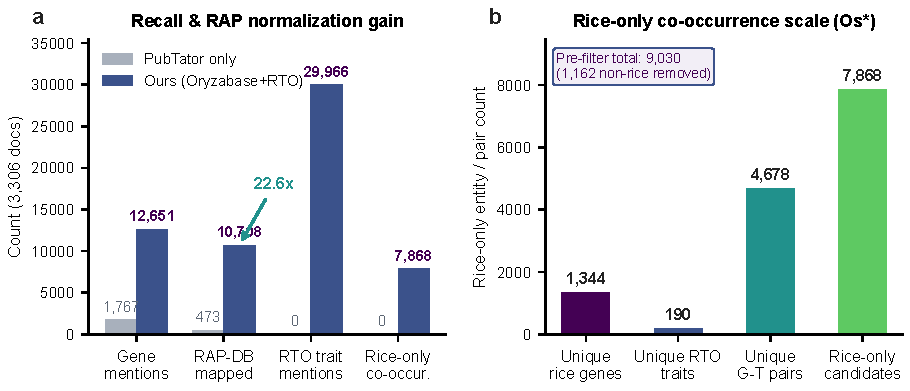
\includegraphics[width=0.92\textwidth]{figure/fig3_pipeline_ablation.pdf}
  \caption{实体识别消融实验与水稻专有共现规模。(a) PubTator 原生注释与本文 Oryzabase+RTO 流水线在基因映射和性状覆盖上的对比；(b) 按 \texttt{Os*} 前缀过滤非水稻基因后保留的水稻知识库规模（另注明过滤前总候选为 9,030 条）。数据来源：\texttt{part2\_normalization\_and\_evidence\_report.json} 与 \texttt{key\_numbers.json}。}
  \label{fig:ablation}
\end{figure*}

\begin{figure*}[t]
  \centering
  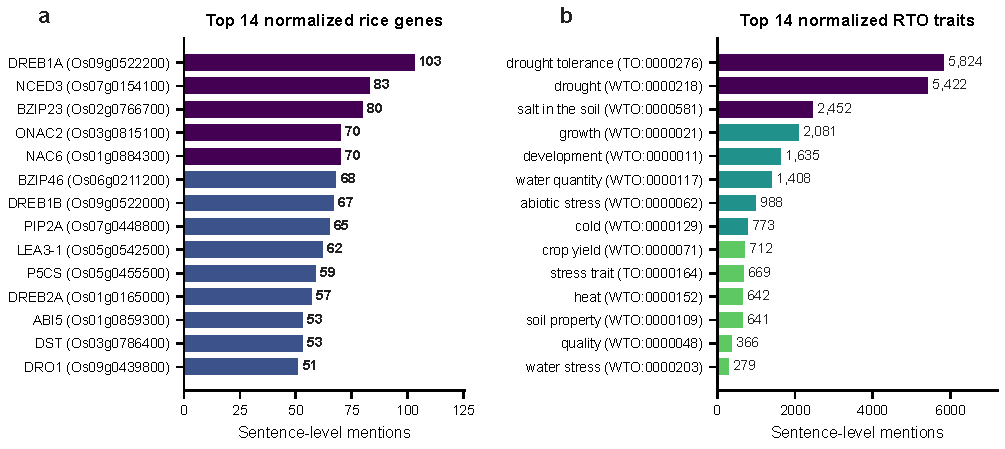
\includegraphics[width=0.95\textwidth]{figure/fig4_top_genes_traits.pdf}
  \caption{归一化后出现频次最高的 Top 14 水稻抗旱基因（附标准 RAP ID）与 Top 14 RTO 性状（附本体编号）。数据来源：\texttt{part2\_normalization\_and\_evidence\_report.json}。}
  \label{fig:top_entities}
\end{figure*}

图~\ref{fig:top_entities} 与表~\ref{tab:top_genes} 列出了出现最频繁的水稻抗旱基因、性状及别名归并情况。排在前 10 位的都是水稻抗旱研究的代表性基因，包括 AP2/ERF 因子 \texttt{DREB1A}（103 次）、ABA 限速酶 \texttt{NCED3}（83 次）、bZIP 转录因子 \texttt{BZIP23}（80 次）、\texttt{ONAC2}（70 次）和 \texttt{NAC6}（70 次）等。比如 \texttt{ONAC2}（\texttt{Os03g0815100}）在原文里有 \texttt{SNAC1}（51 次）、\texttt{OsNAC9}（12 次）、\texttt{OsSNAC1}（6 次）和 \texttt{ONAC2}（1 次）四种写法，经过归一化后全部汇总到同一位点；如果不做别名收敛，同一基因在不同文献里的证据会被拆散。同时也能看到一个残留隐患：排在第 15 位的 \texttt{D1}（\texttt{Os05g0333200}，51 次）在 Oryzabase 里带有一个别名 \texttt{RGA}，容易和表示“根生长角”的英文缩写 \texttt{root growth angle (RGA)} 混淆，在后面的审计里确实引发了误匹配。

\begin{table*}[t]
  \centering
  \footnotesize
  \renewcommand{\arraystretch}{1.05}
  \setlength{\tabcolsep}{4pt}
  \caption{Top 10 水稻抗旱基因的异构别名汇聚与 RAP-DB 归一化结果（数据来源：\texttt{part2\_normalization\_and\_evidence\_report.json}）}
  \label{tab:top_genes}
  \begin{tabularx}{\textwidth}{@{}c l l r p{6.2cm} X@{}}
    \toprule
    排名 & 标准符号 & RAP ID & 提及数 & 语料中自动归并的异构写法（频次） & 基因功能与抗旱角色 \\
    \midrule
    1  & DREB1A & \texttt{Os09g0522200} & 103 & \texttt{DREB1A} (37), \texttt{OsDREB1A} (31), \texttt{CBF3} (24), \texttt{DREB1a} (9), \texttt{Cbf3} (2) & AP2/ERF 转录因子，结合 DRE 顺式元件 \\
    2  & NCED3  & \texttt{Os07g0154100} & 83  & \texttt{OsNCED3} (36), \texttt{OsNCED4} (27), \texttt{NCED4} (10), \texttt{NCED3} (8) & ABA 生物合成关键限速酶 \\
    3  & BZIP23 & \texttt{Os02g0766700} & 80  & \texttt{OsbZIP23} (70), \texttt{osbZIP23} (4), \texttt{OsZIP23} (2), \texttt{OsAREB2} (2) & ABA 依赖型 bZIP 转录因子 \\
    4  & ONAC2  & \texttt{Os03g0815100} & 70  & \texttt{SNAC1} (51), \texttt{OsNAC9} (12), \texttt{OsSNAC1} (6), \texttt{ONAC2} (1) & 调控气孔关闭与根系发育的 NAC 因子 \\
    5  & NAC6   & \texttt{Os01g0884300} & 70  & \texttt{OsNAC6} (40), \texttt{OsNAC2} (14), \texttt{SNAC2} (10), \texttt{NAC6} (3) & 介导根系重构与逆境响应的 NAC 因子 \\
    6  & BZIP46 & \texttt{Os06g0211200} & 68  & \texttt{OsbZIP46} (41), \texttt{OsABF2} (8), \texttt{OsbZIP46CA1} (7), \texttt{ABF3} (5) & AREB/ABF 亚家族成员，正调控抗旱 \\
    7  & DREB1B & \texttt{Os09g0522000} & 67  & \texttt{OsDREB1B} (38), \texttt{DREB1B} (12), \texttt{CBF1} (9), \texttt{OsDREB1C} (7) & 逆境诱导型 DREB 转录因子 \\
    8  & PIP2A  & \texttt{Os07g0448800} & 65  & \texttt{OsPIP2} (49), \texttt{PIP2} (12), \texttt{OsPIP2a} (3), \texttt{OsPIP2-1} (1) & 质膜水通道蛋白，调节根系水力导度 \\
    9  & LEA3-1 & \texttt{Os05g0542500} & 62  & \texttt{OsLEA3} (34), \texttt{OsLEA3-1} (11), \texttt{LEA3} (7), \texttt{Lea3} (4) & 胚胎晚期丰富蛋白，维持逆境结实率 \\
    10 & P5CS   & \texttt{Os05g0455500} & 59  & \texttt{P5CS} (33), \texttt{OsP5CS} (12), \texttt{OsP5CS1} (9), \texttt{P5CS1} (5) & 脯氨酸合成限速酶，参与渗透调节 \\
    \bottomrule
  \end{tabularx}
\end{table*}

\subsection{SDP 因果抽取与 100 条分层人工审计}
在 7,868 条水稻候选共现上，SDP 模块筛出 884 条候选因果调控关系（占 11.24\%）和 1,379 条 \texttt{association}（17.53\%）；其余 5,489 条因为缺少基因到性状的支配路径被归入 \texttt{excluded\_direction}，48 条因 \texttt{respectively} 索引错位被排除，另有 35 条 \texttt{no\_effect} 和 33 条无有效依存路径（表~\ref{tab:sdp_eval}、图~\ref{fig:sdp}）。这 884 条因果涉及 385 个基因、72 个性状和 693 个唯一基因--性状对，分布在 414 篇文献的 647 个句子里。方向分布上，正向调控 575 条、负向 150 条、中性 159 条，正负比为 $3.83:1$；高、中、低置信度分别有 511、200 和 173 条；按句法结构分，主动语态 635 条、链式从句 182 条、轻动词形容词 64 条、被动语态 3 条；其中 loss-of-function 极性反转规则实际生效 73 条（其余为基因直接主语 557 条、gain-of-function 254 条）。在 72 条满足并列列表长度的 \texttt{respectively} 句子里，规则保留了 24 条对齐正确的配对，拦掉了 48 条错配。

\begin{figure*}[t]
  \centering
  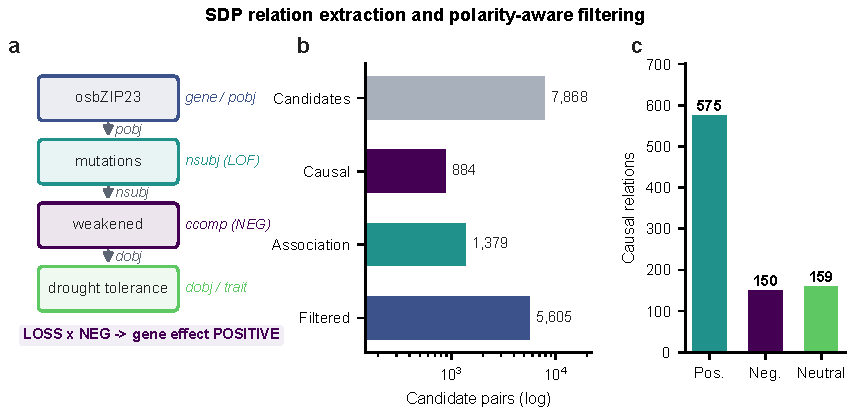
\includegraphics[width=0.92\textwidth]{figure/fig5_sdp_framework.pdf}
  \caption{SDP 因果关系抽取示例与过滤分布。(a) \texttt{osbZIP23} 突变降低耐旱性的依存路径，loss-of-function 构建与负向谓词叠加后还原为正向调控；(b) 7,868 条水稻候选对的分流统计；(c) 884 条候选因果关系的极性构成。数据来源：\texttt{sdp\_relations.tsv} 与 \texttt{sdp\_summary.json}。}
  \label{fig:sdp}
\end{figure*}

\begin{table*}[t]
  \centering
  \footnotesize
  \renewcommand{\arraystretch}{1.05}
  \setlength{\tabcolsep}{6pt}
  \caption{SDP 全量关系判定分布（$n=7{,}868$）与 100 条分层人工审计指标（数据来源：\texttt{sdp\_summary.json} 与 \texttt{sdp\_audit\_summary.json}）}
  \label{tab:sdp_eval}
  \begin{tabularx}{0.96\textwidth}{@{}l r r @{\hspace{14pt}}|@{\hspace{14pt}} X r@{}}
    \toprule
    \multicolumn{3}{c}{SDP 全量判定分布（$n=7{,}868$）} & \multicolumn{2}{c}{100 条分层人工审计（A 层 50 + B 层 50，seed=42）} \\
    关系类别 & 数量 & 占比 & 评测指标 & 数值 \\
    \midrule
    \texttt{positive\_regulation} & 575 & 7.31\% & SDP 精确率（A 层 $43/50$） & 86.0\% \\
    \texttt{negative\_regulation} & 150 & 1.91\% & 精确率 95\% Wilson 置信区间 & 73.8\%--93.0\% \\
    \texttt{regulation}（中性）    & 159 & 2.02\% & 共现基线精确率（分层加权） & 34.5\% \\
    因果调控小计                  & 884 & 11.24\% & 分层外推召回率 / $F_1$（基线 $F_1=0.51$） & 28.0\% / 42.2\% \\
    \texttt{association}          & 1,379 & 17.53\% & 预期真实因果数（TP 估算） & $\approx 760$ 条（760.2） \\
    \texttt{excluded\_direction}  & 5,489 & 69.76\% & 极性判别准确率（$30/34$） & 88.2\% \\
    \texttt{excluded\_respectively}& 48   & 0.61\% & 极性混淆（正对/负对/正错/负错） & 23 / 7 / 2 / 2 \\
    \texttt{no\_effect} / \texttt{unsupported} & 68 & 0.86\% & 误判统计（A 层 FP / B 层 FN / 极性冲突） & 7 / 14 / 4 \\
    \bottomrule
  \end{tabularx}
\end{table*}

100 条分层人工审计把精度和召回率的取舍摆得很清楚（表~\ref{tab:sdp_eval}、图~\ref{fig:eval}a）：A 层 50 条样本中 43 条确认为真实调控，精确率为 86.0\%（95\% CI: 73.8\%--93.0\%），比加权共现基线（34.5\%）高出 51.5 个百分点，按此估算 884 条候选因果中大约有 760 条为真实调控关系；在 34 条方向明确的样本里极性准确率达到 88.2\%（30/34）。不过由于规则卡得比较严，分层外推召回率只有 28.0\%（$F_1=42.2\%$，低于共现基线 $F_1=0.51$），说明它更适合用来挑高可信调控边，而不是替代全量召回。

\begin{figure*}[t]
  \centering
  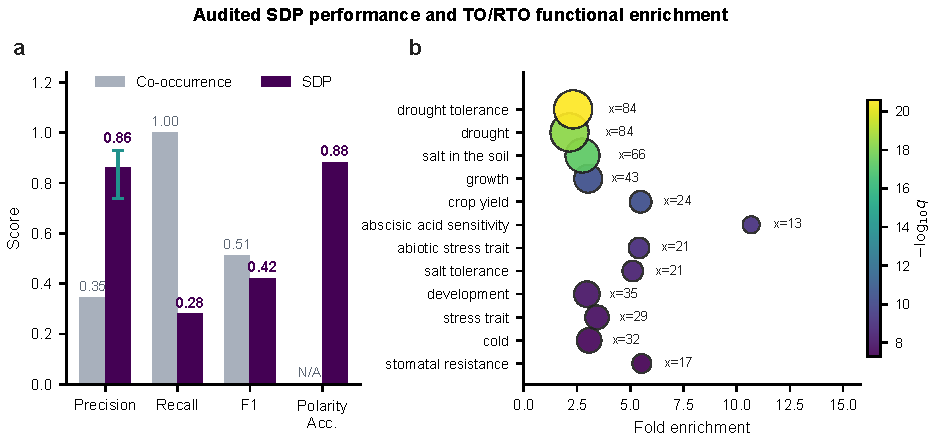
\includegraphics[width=0.92\textwidth]{figure/fig6_evaluation_enrichment.pdf}
  \caption{SDP 审计性能对比与功能富集分析。(a) 100 条分层审计中，共现基线与 SDP 在精确率、召回率、$F_1$（基线 0.51）和极性准确率（SDP 0.88）上的对比；(b) Top 100 SDP 因果基因集中显著富集的前 12 个 TO/RTO 条目（气泡大小对应命中基因数 $x$，颜色对应 $-\log_{10} q$）。数据来源：\texttt{sdp\_audit\_summary.json} 与 \texttt{part4\_enrichment\_summary.json}。}
  \label{fig:eval}
\end{figure*}

表~\ref{tab:audit_cases} 挑出了 10 条有代表性的审计原文（包括 4 条正确样本、4 条 A 层误判和 2 条 B 层漏检）。正确样本说明直接调控、\texttt{respectively} 对齐（A36）以及 \texttt{knockout}/\texttt{silencing} 反转（A46、A13）都能稳定工作。7 条 A 层假阳性和 4 条极性冲突则集中出在五种情况：（1）字母缩写碰撞，如 A01 把根生长角 \texttt{RGA} 错当成 \texttt{D1}；（2）HTML 标签残留干扰，如 A48 句子里的下标标签 \texttt{log<sub>2</sub>} 被误切成 \texttt{sub}（淹水敏感性）；（3）间接机理，如 A03 调控通道蛋白、A18 抑制耐旱负调控因子；（4）宾语负向名词未反转，如 A04 的 \texttt{increased sensitivity} 实际表示耐旱变差，但系统按 \texttt{increased} 判成了正向；（5）部分功能缺失短语漏触发（A07 的 \texttt{knocking out}、A39 的 \texttt{loss of ... function}）以及并列分句取错谓词（A42）。另外，B 层 14 条假阴性（如表~\ref{tab:audit_cases} 中的 B29 和 B31）大多用了 \texttt{is positively involved in}、\texttt{were markedly tolerant to} 或 \texttt{showed enhanced tolerance} 这类轻动词或评价形容词句式，当前规则还没有收全，目前大多留在 \texttt{association} 或 \texttt{excluded\_direction} 池里。

\begin{table*}[t]
  \centering
  \scriptsize
  \renewcommand{\arraystretch}{1.04}
  \setlength{\tabcolsep}{3.5pt}
  \caption{100 条分层人工审计的代表性正确、A 层误判与 B 层漏检案例（数据来源：\texttt{table10\_sdp\_audit\_100.csv}）}
  \label{tab:audit_cases}
  \begin{tabularx}{\textwidth}{@{}c l l c c X@{}}
    \toprule
    ID & 基因 / 性状 & SDP 输出 & Gold & 极性 & 诊断归类与原文证据（节选） \\
    \midrule
    A02 & \texttt{SST} / \texttt{salt} & \texttt{negative} & $-1$ & $\checkmark$ & 正确（直接负调控）：\textit{OsSPL10 ... negatively regulate salt and drought stress tolerance in rice.} \\
    A46 & \texttt{PRX130} / \texttt{drought tolerance} & \texttt{positive} & $+1$ & $\checkmark$ & 正确（LOF 反转）：\textit{Knockout of OsPRX130 ... compromising the drought tolerance in rice.} \\
    A13 & \texttt{GRX22} / \texttt{drought tolerance} & \texttt{negative} & $-1$ & $\checkmark$ & 正确（LOF 反转）：\textit{Silencing of OsGRXS17 in rice improves drought stress tolerance.} \\
    A36 & \texttt{BHLH148} / \texttt{drought tolerance} & \texttt{regulation} & \texttt{reg} & -- & 正确（\texttt{respectively} 对齐）：\textit{...OsbHLH148 and OsBIHD1, which regulate drought tolerance and blast defense, respectively.} \\
    A01 & \texttt{D1} / \texttt{water quantity} & \texttt{regulation} & $0$ & -- & FP（缩写同形）：\textit{The root growth angle (RGA) ... affects the area in which roots capture water...} \\
    A04 & \texttt{PFA-DSP1} / \texttt{drought tolerance} & \texttt{positive} & $-1$ & $\times$ & 极性错（敏感性名词）：\textit{Ectopic overexpression of OsPFA-DSP1 ... increased sensitivity to drought stress.} \\
    A07 & \texttt{GSTU17} / \texttt{drought tolerance} & \texttt{negative} & $+1$ & $\times$ & 极性错（LOF 漏命中）：\textit{...knocking out OsGSTU17 significantly reduced the drought tolerance...} \\
    A42 & \texttt{PP2C49} / \texttt{crop yield} & \texttt{negative} & $+1$ & $\times$ & 极性错（取错并列分句）：\textit{OsPP2C49 overexpression led to decreased ABA sensitivity and increased rice grain yield...} \\
    B29 & \texttt{PUB67} / \texttt{drought tolerance} & \texttt{excluded\_dir.} & \texttt{reg} & -- & FN（轻动词+介词）：\textit{A U-box E3 ubiquitin ligase OsPUB67 is positively involved in drought tolerance in rice.} \\
    B31 & \texttt{WSI76} / \texttt{drought tolerance} & \texttt{excluded\_dir.} & $+1$ & -- & FN（系动词+形容词）：\textit{Transgenic rice plants, in which ... OsGolS2 were constitutively expressed, were markedly tolerant to ...} \\
    \bottomrule
  \end{tabularx}
\end{table*}

\subsection{TO/RTO 功能富集、RiceMind 注释缺口与基因--性状网络}
在 2,218 个背景基因和 272 个 TO/RTO 条目中，SDP 因果证据排名前 100 的基因一共命中 151 个条目，其中 53 个达到 BH 校正显著水平（$q<0.05$，图~\ref{fig:eval}b）。除了命中数排在最前的 \texttt{drought tolerance}（$x=84/100$，富集 2.32 倍，$q=2.58\times 10^{-21}$）、\texttt{drought}（84，2.15 倍，$q=5.51\times 10^{-19}$）和 \texttt{salt in the soil}（66，2.76 倍，$q=5.99\times 10^{-18}$）外，与核心抗旱生理直接相关的 \texttt{abscisic acid sensitivity}（$x=13$，10.68 倍，$q=7.86\times 10^{-10}$）、\texttt{grain size}（$x=8$，8.87 倍，$q=2.02\times 10^{-5}$）和 \texttt{stomatal resistance}（$x=17$，5.54 倍，$q=5.22\times 10^{-8}$）富集倍数最高。作为对照，Top50 与 Top20 查询集分别显著富集 46 和 40 个条目；而基于高频文献预先挑出的 14 个核心基因虽命中 68 个条目，但自带筛选偏倚，所以主文只以 Top100 结果作为依据。

把这 100 个基因放到 RiceMind 里交叉比对（表~\ref{tab:ricemind}），能查到 99 个标准 RAP 记录（覆盖率 99\%），其中 85 个带有一般的 \texttt{stress/tolerance} 注释，但只有 13 个在 \texttt{annotation} 里明确写到了 \texttt{drought/water deficit}（5 个写到了 ABA）。按“至少有 3 个唯一 SDP 因果对且 RiceMind 里没有抗逆注释”这一条件筛选，一共挑出 13 个注释缺口候选（前 5 名为 \texttt{DRAP1}、\texttt{ANN1}、\texttt{CALA}、\texttt{BHC} 和 \texttt{Os01g0178600}）。要特别说明的是，这些基因已有文献报道，并不是新发现基因，它们代表的是公共库里还缺少抗逆或干旱注解、值得优先人工审编的对象。

最后，把 693 个唯一因果基因--性状对拼在一起，得到一个包含 457 个节点和 693 条无向汇总边的二分网络（图~\ref{fig:network}）。性状端里 \texttt{drought tolerance}（加权度 286、度 196）、\texttt{drought}（119、93）和 \texttt{salt in the soil}（102、71）连边最多，接着是 \texttt{growth}（47）、\texttt{crop yield}（24）和 \texttt{stomatal resistance}（22）；基因端排在最前的是 \texttt{DSR2}（加权度 15）、\texttt{ONAC2}（10）、\texttt{WOX11}（9）、\texttt{HDA704}（9）和 \texttt{OsMYB4}（9）。这些连边汇总的是文献句子数，只反映哪些基因--性状在语料里被重复报道得多。

\begin{table}[t]
  \centering
  \footnotesize
  \renewcommand{\arraystretch}{1.04}
  \setlength{\tabcolsep}{2.5pt}
  \caption{Top 100 基因 RiceMind 覆盖情况与注释缺口候选 Top 5（数据来源：\texttt{table13} 与 \texttt{table15}）}
  \label{tab:ricemind}
  \begin{tabularx}{\columnwidth}{@{}l r @{\hspace{5pt}}|@{\hspace{5pt}} l l c X@{}}
    \toprule
    \multicolumn{2}{c}{RiceMind 覆盖统计} & \multicolumn{4}{c}{缺口候选（$\ge 3$ 对且无 stress 注释）} \\
    统计项 & 数值 & 基因 & RAP ID & 对数 & 主要 SDP 性状 \\
    \midrule
    查询数 & 100 & DRAP1 & \texttt{Os11g0544700} & 5 & drought tol.(2), salt(1) \\
    找到记录 & 99 (99\%) & ANN1 & \texttt{Os01g0497400} & 4 & stress(1), heat(1) \\
    含 stress & 85 & CALA & \texttt{Os05g0491100} & 4 & abiotic(1), heat(1) \\
    含 drought & 13 & BHC & \texttt{Os04g0624500} & 4 & stomatal(2), salt(2) \\
    缺口候选 & 13 & -- & \texttt{Os01g0178600} & 4 & drought(1), tol.(1) \\
    \bottomrule
  \end{tabularx}
\end{table}

\begin{figure}[t]
  \centering
  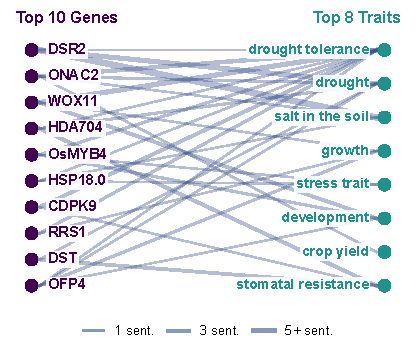
\includegraphics[width=0.96\columnwidth]{figure/fig7_gene_trait_network.pdf}
  \caption{基于 SDP 因果关系汇总的基因--性状加权二分网络核心子图（展示连接度最高的 Top 10 基因与 Top 8 性状；全网络共 457 节点、693 条无向边，边宽反映去重证据句数）。数据来源：\texttt{part4\_network\_nodes.csv} 与 \texttt{edges.csv}。}
  \label{fig:network}
\end{figure}

% ======================================================================
%  V. 讨论 Discussion
% ======================================================================
\section{讨论 Discussion}

\subsection{结果意味着什么 Implications}
这几组实验对照把作物文献挖掘里容易踩坑的地方摆得比较清楚。检索词确实不能全凭经验拍板：\texttt{drought stress} 比 \texttt{drought tolerance} 多覆盖了 41.9\% 的文献，检索式一旦写窄，后面换再复杂的抽提模型也补不回来。农学实体归一化也是同样的情况：Oryzabase 让基因覆盖量翻了二十多倍，但同时带进了 \texttt{ha-1} 和 \texttt{Apo} 这类冲突词；必须配合黑名单，再在共现后按 \texttt{Os} 前缀剔除 1,162 条外源共现，单物种知识图谱的口径才不会乱。

共现和因果也不用硬二选一。SDP 把精确率拉到了 86.0\%，代价是只找回了不到三成的真实调控；把高可信因果放进主干网络，其余 1,379 条 \texttt{association} 留在补充层里给检索和人工核查用，实际用起来更稳妥。RiceMind 里有 85 个基因带一般抗逆注释，却只有 13 个明确写出了干旱，这也说明文献挖掘的主要用处在补全具体胁迫表型注解，而不是重找早已发表过的基因。

\subsection{局限性与误差边界 Limitations}
对照误判和漏检例子，用这批数据时还得注意几处边界。前端词典和文本清洗仍有残留噪音：静态词典压不住全部多义缩写，比如 \texttt{RGA} 既指基因 \texttt{D1} 也指根生长角（A01），\texttt{SAMs} 会撞上 \texttt{SAMS1}；A48 里的 \texttt{log<sub>2</sub>} 没洗掉 HTML 标签，里面的 \texttt{sub} 就被误切成了淹水敏感性。遇到短缩写或残留格式标签的句子，入库前还得人工复查。

规则的覆盖度和方向判定也留有盲区。28.0\% 的召回率代表不少真实调控句子没进因果层，常见漏检是 \texttt{is positively involved in}、\texttt{were markedly tolerant to} 这类轻动词和形容词句式（B29、B31）。方向判别上错的 4 条（4/34）则来自 \texttt{increased sensitivity}（A04）、漏触发的敲除短语（A07、A39）和并列分句取错谓词（A42）。此外，100 条审计为分层采样且由作者配合 Agent 预标复核，尚缺多专家双盲标注；5 篇 2026 年论文因 PubTator 未索引也未入主统计。TO/RTO 富集只说明基因集整体落在抗旱通路上，不能替代单条关系的实验证实，而图~\ref{fig:network} 的节点度也只累加了证据句数。

\subsection{下一步工作 Future Work}
把错因逐条拆开后，后面的改进也就比较好落地。近期可以直接修两处规则与清洗漏洞：先从摘要里剥掉 \texttt{<sub>}、\texttt{<i>} 等 HTML 标签，再把 \texttt{markedly tolerant to}、\texttt{positively involved in}、\texttt{showed enhanced [trait]} 补进句法模式，配合 \texttt{sensitivity/susceptibility} 极性反转词表和分句边界约束，修掉 A04、A42 和 B 层漏检。再往后，用 511 条高置信因果句和已核出的负例作弱监督数据，去微调 PubMedBERT 等轻量生物医学分类器，重点补回 B 层里散落的隐含调控句并守住 85\% 以上精确率。对于表~\ref{tab:ricemind} 的 13 个 RiceMind 注释缺口候选（如 \texttt{DRAP1}、\texttt{ANN1} 和 \texttt{BHC}），则需要逐篇调出原文人工核实并对照转录组与突变体表型补全注解。

% ======================================================================
%  VI. 结论 Conclusion
% ======================================================================
\section{结论 Conclusion}

面向水稻抗旱文献中的检索漏检、农艺性状缺口和共现噪声问题，本文完成了一套从 PubMed 摘要抓取到知识库审计的流程。我们在 3,306 篇全文（795,401 词元）上合并 Oryzabase、RTO-1.0 与五条农学消歧规则，把 RAP 水稻基因归一化提升到 PubTator 原生映射的 22.6 倍，过滤非水稻记录后保留 7,868 条水稻候选对；再用 spaCy 最短依存路径联合极性、否定和 \texttt{respectively} 对齐规则，从中抽取出 884 条候选因果关系（693 个唯一对）和 1,379 条 \texttt{association}。100 条分层人工审计测得 SDP 精确率为 86.0\%（95\% CI: 73.8\%--93.0\%）、极性准确率 88.2\%、召回率 28.0\%；Top100 因果基因在 TO/RTO 中有 53 个条目显著富集，并在 RiceMind 中挑出 13 个还没补全抗逆注释的审编候选基因，为后续建设可核查的水稻抗旱知识图谱准备好了数据和代码基础。

% ======================================================================
%  数据与代码可用性
% ======================================================================
\section*{数据与代码可用性 Data and Code Availability}
全部实验脚本（\texttt{scripts/01}--\texttt{12}）、一键重跑入口 \texttt{run\_all.py}（复用本地语料约 1.5 分钟跑完）与中间结果均保存在 GitHub 仓库 \url{https://github.com/ZimingADR/BioNLP}。主要交付表格包含 \texttt{rice\_drought\_sentence\_evidence.tsv}（9,030 条总候选，含 7,868 条水稻专有对）、\texttt{sdp\_relations.tsv}（884 条候选因果与 1,379 条 \texttt{association}）、\texttt{sdp\_audit\_labels.json}（100 条审计标签）以及 \texttt{part4\_novel\_targets.csv}（13 个注释缺口候选），全部字符偏移均通过 \texttt{text[b:e]==mention} 校验。

% ======================================================================
%  致谢
% ======================================================================
\section*{Acknowledgment 致谢}
感谢华中农业大学《生物文本挖掘与知识发现》课程以及夏静波老师在选题与方法设计上的指导；感谢 Oryzabase、RAP-DB、RiceMind、RTO 与 PubTator 团队开放的数据与接口。文中实验口径、核心指标核查和全部学术判断均由作者本人完成审查，AI Agent 仅用于辅助脚本编写、数据整理与初稿起草。

% ======================================================================
%  参考文献
% ======================================================================
\IEEEtriggeratref{9}
\bibliographystyle{IEEEtran}
\bibliography{reference}

\end{document}
